\chapter{METHODOLOGY}
\label{ch:methodology}

In this section, we provide detail about the experiment detail, which investigates the effectiveness of combining text and image representation for the self-distillation method.
We divide the methodology section into 3 sections.
First, the model architecture section provides the image-text representation head and teacher-student model detail.
Second, the training objective is described in this section.
The third section is evaluation method.
In the last section, we provide in depth ablation study.

\section{Model Achitecture}
\subsection{Image-text representation head}
By using two encoder model for vision and language individually, the image-text representation have be created to get a single image representation for every single images.
In this experiment, the cross-attention \shortcite{alayrac2022flamingo} architecture with the linear classification head is used to create image-text representation as illustrated in Figure \ref{fig:cross_attention}.

\begin{figure}[h]
\caption{Image-Text Cross Attention Classification head}
\label{fig:cross_attention}
\centering
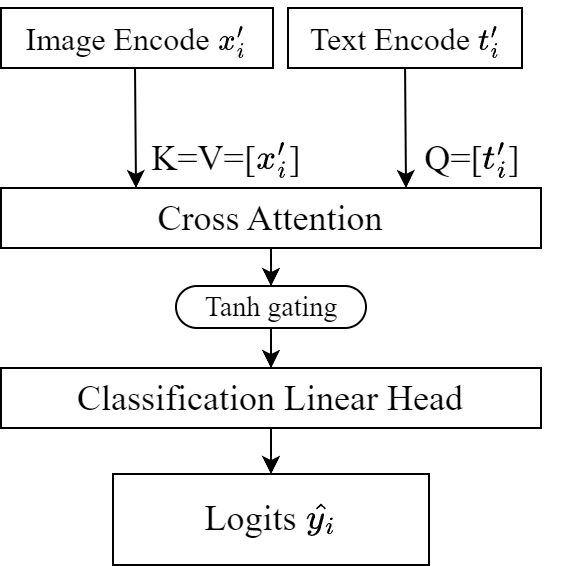
\includegraphics[width=0.5\textwidth]{Images/CrossAttention.png}
\end{figure}

\subsection{Teacher student}
For the teacher model, we will use two stream encoder based model same as CLIP model \shortcite{dosovitskiy2021an}.
In this experiment, the teacher vision encoder model will be ResNet \shortcite{he2016deep} and ViT \shortcite{dosovitskiy2021an} version.
For the student model we used the same architecture as teacher vision encoder model, which are ResNet and ViT.
\textcolor{red}{todo: Add table describes both image and text encoders.}

\section{Training Objectives}
In the first step, we trained the image-text representation head with benchmark datasets by using Cross Entropy loss as describe in \ref{fig:overall_method} a). The image and text encoder was freezed during the first step training. For text input, we used "This is the image of [Class]" as a prompt \shortcite{radford2021learning}. After the first image-text representation head were trained, we create a new student model which have the same architecture as a image encoder model with a linear classification head. The student model was randomly initialized parameters. The objective for self-distillation with teacher and student is  

\begin{figure}[h]
\caption{Training methodology}
\label{fig:methodology}
\begin{center}
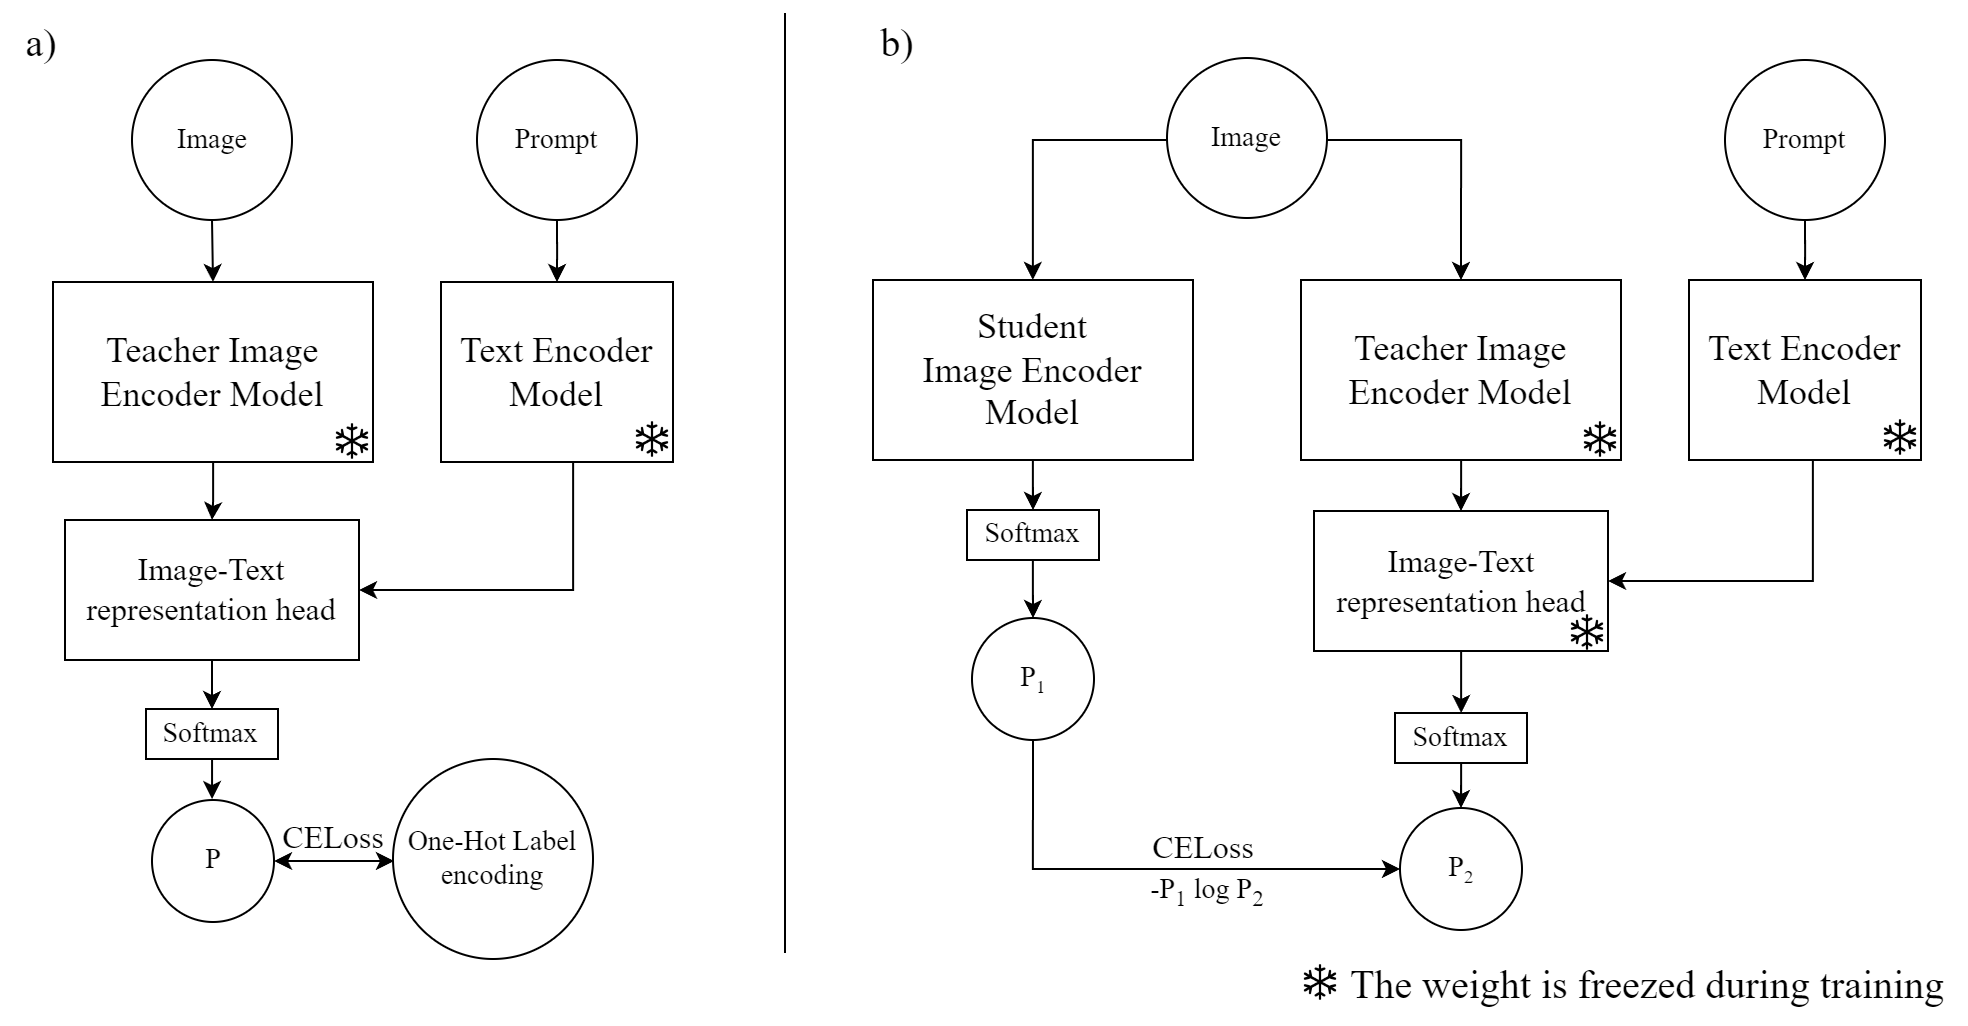
\includegraphics[width=1\textwidth]{Images/Methodology.png}
\end{center}
\small a) Training image-text representation head using cross entropy loss b) Self-distillation training by freezing all teacher model
\end{figure}

\section{Evaluation}
\section{Ablation Study}

